\section{Security honeypot}
\label{sec:honeypot}

The ability to perform parallel multi-version execution could be also used to
deploy high-interaction honeypots that can offer a detailed account of the
attackers' activities. These honeypots could run vulnerable versions of
security critical services, and compare their behaviour, in real time, against
that of a known secure version.  Any divergence detected could be resolved in
favour of the secure version and logged for further analysis.  This would
provide a fine-grained understanding of the anatomy of an attack, which is
typically not possible with today's honeypot deployments. The construction
of such a honeypot system using an existing multi-variant execution
environment has been already proposed in the past~\cite{jackson10} but,
to our knowledge, no implementation of such mechanism exists.
%The use of multi-variant execution to construct such honeypot systems has been
%already proposed in the past~\cite{jackson10}. However, to our knowledge, no
%general-purpose implementation of such mechanism exists.

We have implemented this security mechanism in a simple prototype system based
on top of \varan~\cite{pes:mvh}. This system runs two variants of an
application---\emph{public} and \emph{private}---in lockstep and monitors their
behavior. A monitor synchronises the execution of the two variants and grants
or denies access to operating system resources. Any divergence in the variant
behavior might be a sign of an ongoing attack. While this prototype reuses a
large part of the \varan's codebase, namely the preloader, the monitor and the
system call interception mechanism, there are several important differences.

In a regular multi-variant or multi-version application, all versions run on
the same machine under the same security restrictions.  However, in the
honeypot system, each variant has a different access to operating system
resources such as file system and network.

For example, consider a web service running on top of the multi-variant
honeypot (MVH). A public variant is granted access to network resources while
the private variant can only access the file system. Every request received by
the public variant is forwarded to the private variant through the monitor, and
after being processed, the result is sent back to the public version. When the
public version is compromised due to an existing (potentially unknown)
vulnerability, it might issue an additional system call in an attempt to
access local resources; this will result in a divergence which will be detected
and recorded by the monitor. The monitor will also close the connection to the
private variant to protect any critical resources.

\begin{figure}[t]
  \begin{center}
    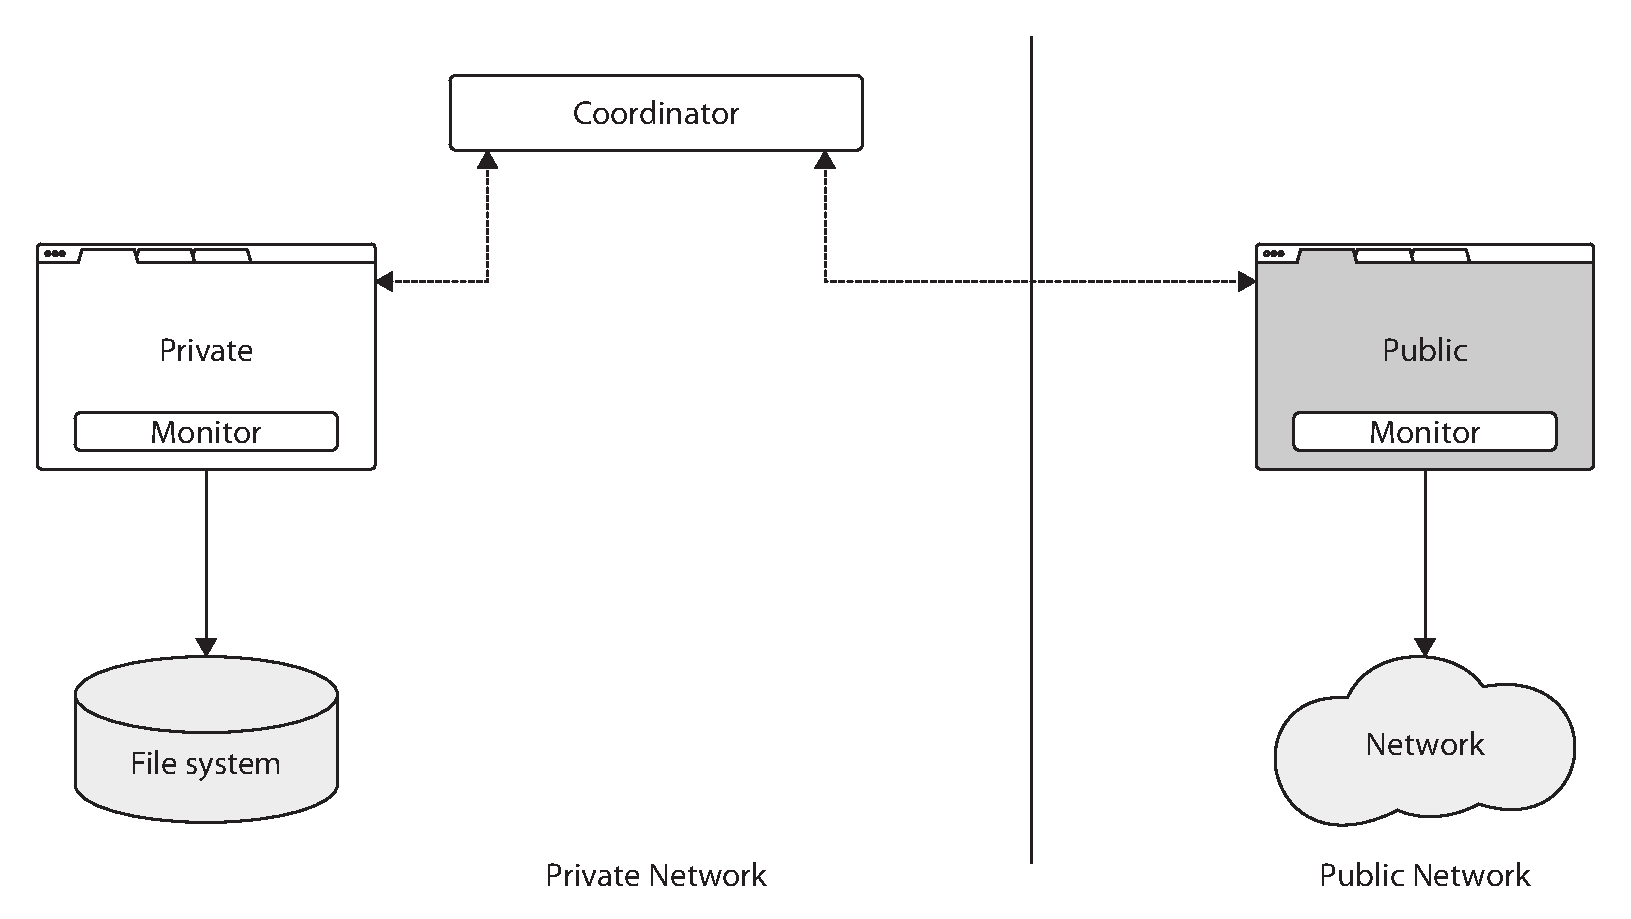
\includegraphics[width=0.75\columnwidth]{applications/figures/honeypot}
    \caption{The architecture of the multi-variant honeypot system.}
    \label{fig:security-honeypot}
  \end{center}
\end{figure}

The architecture of our prototype system is depicted in
Figure~\ref{fig:security-honeypot}.  To enforce strong separation, each variant
can be run on a different machine. Even if attackers manage to subvert our
monitoring infrastructure and gain full access to the operating system, the
impact of such an intrusion can be minimal as the machine which runs the public
version would not contain any critical resources and would ideally be running
inside a demilitarized zone (DMZ) to prevent access to other machines on the
network.  Such an architecture, however, precludes the use of the shared ring
buffer and the streaming architecture (\S\ref{sec:streaming}). Instead, in our
prototype, we use network sockets to transfer events between variants and the
monitor. This has a negative impact on the performance; we have observed a
per-system call overhead of \numrange{18}{25}$\times$ in our microbenchmarks.
However, we believe that in the case of honeypot systems, performance overhead
is not the most important factor, as the applications running on top of such
systems are not expected to be used in performance critical scenarios.

We have tested our prototype by running two variants of \lighttpdgen 1.4.28 on
top of our honeypot system, where the private variant has been compiled with
all the security mechanisms provided by GCC enabled, while the public variant
did not use any of these.
%\footnote{We used \lstinline`-fstack-protector-all -Wstack-protector --param
%ssp-buffer-size=4 -pie -PIE -ftrapv -D_FORTIFY_SOURCE=2 -z relro,now` GCC
%options for the private variant and \lstinline`-fno-stack-protector -z
%execstack` options for the public variant.}
We then used an existing exploit~\cite{erickson:hacking-networking} to attack the public variant and
inject shellcode\footnote{\url{http://www.shell-storm.org/shellcode/files/shellcode-658.php}}
which tries to add a root user with a custom password to the system. This
attack has been successfully detected and prevented by the honeypot monitor.
